\chapter{Create and export your keys}

Let's go ! You're going to do your first real action to use GPG :
generate your first key.\\Or more exactly, your first key pair. Remind
that every GPG key has actually two sides : a public and a private side.

\textbf{This article might look long, but it's an important one.
Creating keys takes a few minutes and you have almost nothing to do. So
please, take your time.}

\subsection{Notice}\label{notice}

NB : for those who are affraid, or concerned about privacy, that I
gather a lot of mail addresses, it's no big deal to me that you use a
fake address for your mail and keys.

After all, it's what I do with the tutorial's address. At the end of the
tutorial, you can create a new key on your real address, follow again
all the various steps.

But you won't send it to me: instead, you will use it for real ! And I
am happy of that !

\subsection{Let's generate the key.}\label{lets-generate-the-key.}

Open your keys manager : Kgpg, Kleopatra or Enigmail (or another
one\ldots{}) and look for the option to create new keys.

With
\href{https://docs.kde.org/stable/en/kdepim/kleopatra/index.html}{Kleopatra
- link to the documentation}, it is \textbf{\emph{Files \textgreater{}
New certificate\ldots{} \textgreater{} Create a personal OpenPGP key
pair}}.

With \href{https://docs.kde.org/stable/en/kdeutils/kgpg/}{Kgpg - link to
the documentation}, it is \textbf{\emph{Keys \textgreater{} Generate key
pair}}.

With Enigmail (inside Thunderbird itself), it is \textbf{\emph{Enigmail
\textgreater{} Key Management}}. Then select \textbf{\emph{Generate
\textgreater{} New Key Pair.}}

\subsubsection{Which address to indicate}\label{which-address-to-indicate}

The software will ask you which address to use with your key.

You can actually set several addresses on a key, but now, better not to
do complicated and set just one.

\subsubsection{Key type}\label{key-type}

Perhaps you will be proposed several algorithmes : DSA \& ElGamal, RSA
or RSA and RSA.

Choose RSA and RSA. It is the strongest combinaison and allows to sign
and encrypt. In Enigmail (tab \emph{advanced}), you'll simply choose
RSA.

\subsubsection{Key size}\label{key-size}

It will ask for a size : 1024, 2048 or 4096 bits. Basically, the larger
the key size, the stronger the key, the longer it is to create the key.
The software will then request to your operating system's \emph{random
generator} some \emph{entropy} of this size.

\begin{quote}
I must admit that I don't understand the whole thing there. As soon as I
try to figure out this entropy, entropy size, I am out ! But I
understood very well that, the more entropy you have, the stronger the
key !
\end{quote}

Today, 4096 bits is the recommanded value.

The key generation will take some time. You mustn't worry or stop the
software.

You can reduce this time using your computer ! The more you use your
computer (particularly hard drives access, called \emph{I/O access} in
geek jargon), the more you generate entropy for your key ! Isn't that
fun ? The good is then to update/upgrade your Linux distribution (high
use of the hard drive) and to look at the last kitten video on
\href{https://vimeo.com/tag:cat}{vimeo}.

\subsubsection{Time expiry}\label{time-expiry}

It's a good idea to set a time expiry.

If you loose access to your key, it will be marked invalid after the
alloted time.

What I do is set a one year validity, and around one month before, push
it away to one more year.

\subsubsection{Passphrase}\label{passphrase}

A \emph{passphrase} is a really long password. For example fifteen or
twenty characters.

There is several methods to create a strong password.

\href{https://xkcd.com/936/}{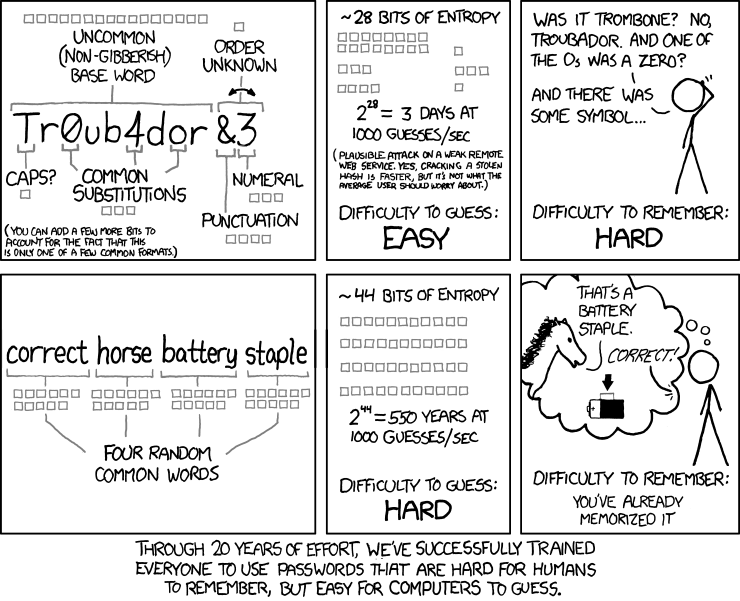
\includegraphics{http://imgs.xkcd.com/comics/password_strength.png}}

\emph{Bonus for foreigners} :\\Use a pretty complicated word of your own
language to start your password. This way, surrounding humans may have
problems finding it !

What I do is that I take a word in my immediate environnement or a
concept that I think of, and then I replace characters in : A becomes @,
l becomes 1 or !, I add numbers\ldots{} One or two changes like this and
the password is strong enought.

\subsubsection{What for a passphrase ?}\label{what-for-a-passphrase}

You can choose not to set a passhprase. I must admit I did not do it for
long. Today I do and recommend it. It simply adds another security.

If you are not the only one to use your computer, or if you use GPG on
your phone or your tablet (often unlocked on the table) then you ought
to set a passhprase.

\subsubsection{Revocation certificate}\label{revocation-certificate}

It is a really good idea to create a revocation certificate, and the key
manager should ask for it.

In case you lose your key, corruption, or someone steal your private
key, then you just publish it on the keys servers. With the updates of
keys servers, the key is declared as invalid quite fast.

This is a safety in case you got some troubles with the private key.

If you just want to change your key in a proper manner, this is not at
all the good way. I will tell you more in a future article.

\subsection{Exercise}\label{exercise}

I thought this tutorial pedagogic from the beginnig. So I am going to
make some little exercises there and now. I created a mail address on my
server for the various purpose of this tutorial, and some keys to play
with.

\textbf{\emph{These keys will never used for anything else than this
tutorial.}}

I will ask you to just send your public key to the mail address. This is
what some people do to exchange keys. Yet there are other ways, but this
topic is for a future article.

After I received your key in mail, I will answer you saying if your keys
has the correct characteristics. I also need it for the next article.

\subsubsection{To export your key}\label{to-export-your-key}

To send me your key, you have to \emph{export} it.

In order to do so, you have to ask your keys manager.

You have to be carefull, as your keys manager can export the whole pair,
public and private.

I ask here for your \textbf{public} key !

As said before, and as its name state it, the public key is available to
anyone. The keys manager will propose you to export your key as a
\emph{gpg} or \emph{asc} file.

This file is actually a raw text file, containing the key itself, which
is a long string of characters. You can edit it with a text editor, like
Notepad or another.

\emph{And no, Word and OpenOffice are not text editors!}

\textbf{\emph{Carefull: if you open the file, don't modify it!}}

Then send it to me as attached file in mail to \emph{Tuto-gpg @
22decembre.eu}.

\emph{NB: Kmail (mail client in KDE) propose also in its menu
}\textbf{Attach\ldots{}} to send your own public key. So simple.